\documentclass[a4paper,11pt]{article}

\usepackage[utf8]{inputenc}

\usepackage{graphicx}

\usepackage{minted}

\usepackage{semantic}

\begin{document}

\title{
  \textbf{Kapa brädor\\
  \small Programmering II}
}
\author{Axel Karlsson}
\date{VT22 \today}

\maketitle

\section*{Inledning}
Syftet med denna uppgift var att prova på dynamisk programmering. Jag har löst ett optimeringsproblem på två sätt, där en av lösningarna använder dynamisk programmering. Jag har sedan gjort några versioner av den dynamiska algoritmen och jämfört deras prestanda.

\section*{Problemet}
Problemet går ut på att dela en planka i ett givet antal delar till de lägsta priset. Varje uppdelning kostar lika mycket som summan av de två resulterande delarna, till exempel så kostar uppdelningen {\tt [5] -> [2, 3]} 5 enheter. Indatan till algoritmen är en lista, till exempel {\tt [1, 2, 3]}. Algoritmen hittar sedan det billigaste sättet att dela upp en planka med längd {\tt 1 + 2 + 3 = 6} i delar med längderna som specificerades i listan. Algoritmen räknar ut detta genom att prova alla möjliga uppdelningar och sedan jämföra deras kostnader.

\subsection*{Den naiva versionen}
Först implementerade jag en algoritm som inte använde dynamisk programmering. Jag hade inga stora svårigheter med att implementera uträkningsdelen av algoritmen, men det tog ett tag innan jag fick den att skriva ut den resulterande uppdelningen på rätt sätt. Jag löste detta genom att i varje anrop returnera var uppdelningen kostade och den resulterande uppdelningen ({\tt tree} i koden nedan). Denna uppdelning skickades sedan vidare ``uppåt'' i rekursionen.
\begin{minted}{elixir}
  # Ett av basfallen för cost/4
  def cost([s], l, [], right)  do
    {cost, tree} = cost(right) # En kostnad och ett träd returneras
    {cost + l + s, {tree, s}} # "Skickar vidare" en kostnad och ett träd
  end
\end{minted}

\subsection*{Map versionen}
I nästa iteration av {\tt cost} implementerades en {\tt map} struktur för att spara värden som redan har räknats. Detta gjorde algoritmen mycket snabbare, det var nu rimligt att lösa problem med fler än tio element. Då jag hade skickat med en träd struktur i den förra versionen var det inte så mycket svårare att skicka en {\tt map} också.
\begin{minted}{elixir}
  # Motsvarande klausul i denna version
  def mcost([s], l, [], right, mem)  do
    {c, t, mem} = mcheck(right, mem)
    {c + l + s, {t, s}, mem}  # Skickar med en map i varje anrop
  end
\end{minted}

\subsection*{Spegelvända mängder}
Nästa förbättring var att undvika att räkna spegelvända mängder flera gånger. I den tidigare versionen hade till exempel {\tt [1, 2, 3]} och {\tt [3, 2, 1]} räknats som olika mängder, fast den resulterande uppdelningen och minsta kostnad är densamma för båda. Detta löstes genom att alltid placera det sista elementet i en sekvens i det vänstra trädet. Koden för detta var given i uppgiften.
\subsection*{Sorterade mängder}
Den sista förbättringen jag gjorde var att sortera varje mängd innan den lades till i {\tt map} strukturen. Detta innebär till exempel att mängderna {\tt [1, 2, 3]}, {\tt [1, 3, 2]} och {\tt [2, 1, 3]} kommer anses som samma mängd vilket bör sänka exekveringstiden. Precis som den förra förbättringen var koden för denna given i uppgiften.

\pagebreak
\section*{Benchmarks}
Jag jämförde de olika versionerna med {\tt bench/1} funktionen som var given i uppgiften. Jag jämförde de fyra tidigare nämnda versionerna (observera att varje version även har de tidigare förbättringarna).
\begin{table}[H]
  \begin{center}
    \begin{tabular}{c|c|c|c|c}
      \textbf{Antal element} & \textbf{Naiv} & \textbf{Map} & \textbf{Vänster} & \textbf{Sorterad}\\
      \hline
      2&1&2&3&4\\
      3&9&8&8&8\\
      4&11&30&20&20\\
      5&110&114&96&78\\
      6&1120&337&220&186\\
      7&15999&900&512&482\\
      8&309508&3864&1536&1470\\
      9&6626622&10744&4684&4675\\
      10&166954608&38197&14539&14443\\
    \end{tabular}
    \caption{Exekveringstid i bench (us)}
    \label{tab:Tabell 1}
  \end{center}
\end{table}
\begin{figure}[H]
  \center
  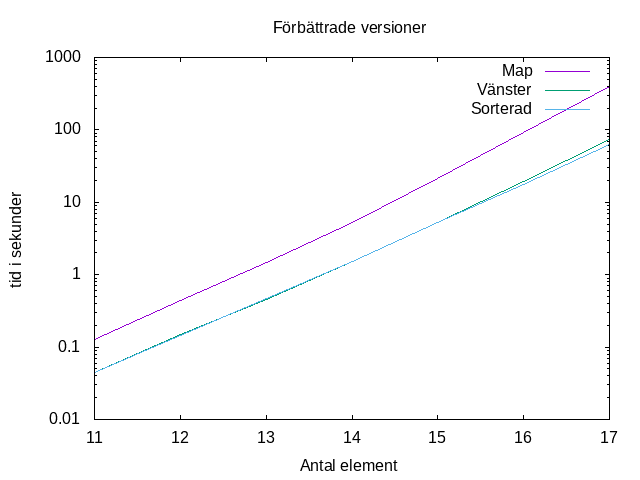
\includegraphics[width=\linewidth]{./latex/images/bench_all_improvments_log.png}
  \caption{Exekveringstid i bench (sekunder). Logaritmisk y-axel.}
  \label{fig:bench_improvements_log}
\end{figure}
\begin{figure}[H]
  \center
  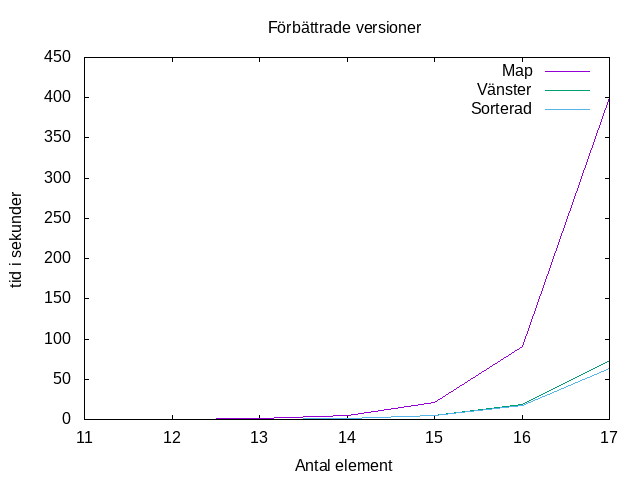
\includegraphics[width=\linewidth]{./latex/images/bench_all_improvments_lin.png}
  \caption{Exekveringstid i bench (sekunder). Linjär y-axel.}
  \label{fig:bench_improvements_lin}
\end{figure}

\section*{Analys} 
I {\tt table 1} ser vi tydligt fördelarna av dynamisk programmering, skillnaden i exekveringstid mellan de versioner med och utan ett minne är enorm. I {\tt figure 2} ser vi även en stor skillnad mellan versionerna som räknar och inte räknar spegelvända sekvenser som olika. Den sista versionen, där alla sekvenser sorterades, verkar inte göra någon skillnad. Detta kan bero på att jag ``bara'' har gjort jämförelsen med 17 element. I uppgiften nämnde Johan att denna förbättring gör större skillnad ju fler element vi räknar med, men då exekveringstiden för varje mätning började närma sig 20 minuter bestämde jag mig för att det räckte. 

\section*{Reflektion}
Jag tycker att denna uppgift var intressant men väldigt lång. Det var en eller två förbättringsförslag i slutet av uppgiften som jag inte han implementera, vilket känns tråkigt. Det hade varit intressant att se hur snabb algoritmen kunde bli.\\
Det är roligt att se hur relativt enkla förändringar kan göra så stor skillnad, och som alltid är man lite mer ödmjuk efter att ha insett hur dåligt den lösningen jag själv hade gjort, den naiva, presterar jämfört med en mer sofistikerad algoritm.
  
\end{document}
